For extensions of the Higgs sector containing two Higgs doublets, the couplings of the heavy Higgs bosons to down-type fermions can be enhanced with respect to the SM for large tan$\beta$ values (the ratio of the vacuum expectation values of the two Higgs doublets).  This results in increased branching fractions to $\tau$ leptons and $b$ quarks, as well as a higher cross section for Higgs boson production in association with $b$-quarks. This has motivated a variety of searches in $\tau\tau$ and $bb$ final states at LEP [29], the Tevatron [30–32] and the LHC -Run1 [33–38], with no indication of an excess over the expected SM background.


The ATLAS collaboration the CMS collaboration have
performed searches for neutral Higgs bosons decaying to $\tau$ leptons using proton--proton collision data collected at a centre-of-mass energy of 13 TeV in 2015, corrisponding to an integrated luminosity
of 3.2 fb$^{−1}$  and 2.3 fb$^{−1}$ respectively. The search is performed in three channels by the  ATLAS collaboration: the $\tau_{e}$$\tau_{\rm had}$ channel where one $\tau$ decays leptonically to an electron and neutrinos and the
other hadronically (to hadrons and a neutrino),  
the $\tau_{\rm \mu}$$\tau_{\rm had}$ channel where the leptonically decaying $\tau$ produce a muon and neutrinos,  and  the  $\tau_{\rm had}$$\tau_{\rm had}$ channel where both $\tau$ leptons decay hadronically. 
In addition to the previos three channels, the CMS collaboration extendeded the search in the $\tau_{e}\tau_{\mu}$ channel  in which both the $\tau$ decay leptonically.
In addition, the CMS collaboriation divided the events into two categories based on the number of b-tagged jets: events with  exactly zero b tagged jets and events with at least one b tagged jet.

\subsection{$\tau_{\rm had}$ reconstruction}
For these analyses, the reconstruction and the identification of hadronic decays of $\tau$ leptons is critical.
The hadronic decays of $\tau$ leptons are predominantly characterized by the presence of one or three charged particles, accompanied by a neutrino and possibly neutral pions. In ATLAS, the reconstruction of their visible decay products, hereafter referred to as $\tau_{\rm had-vis}$, starts with jets reconstructed from topological clusters in the calorimeter using the anti-kt algorithm with a size parameter value $\Delta R = 0.4$ [78]. The $\tau_{\rm had-vis}$ candidate must have energy deposits in the calorimeters in the range $|\eta| < 2.5$, with the transition region between the barrel and end-cap calorimeters ($1.37 < |\eta| < 1.52$) excluded, have a transverse momentum greater than 20 GeV, one or three associated tracks and an electric charge of $\pm1$. A multivariate Boosted Decision Tree (BDT) based identification is used to reject backgrounds from jets, using shower shape and track multiplicity properties of true $\tau_{\rm had-vis}$ objects in the MC. An additional dedicated likelihood-based veto is used to reduce the number of electrons misidentified as $\tau_{\rm had-vis}$. In the ATLAS analysis, two $\tau_{\rm had-vis}$ identification selections are used: "loose" and "medium" with efficiencies for true $\tau_{\rm had-vis}$ objects of about 65\% and 55\%, respectively. In CMS, hadronically decaying $\tau$ leptons are reconstructed using the hadron-plus-strips algorithm [37].
The algorithm considers candidates with one charged pion and up to two neutral pions, or
three charged pions, and is seeded by a jet. The neutral pions decay rapidly into two photons,
and are reconstructed as "strips" of electromagnetic particles, formed with dynamic size
from energy depositions in the electromagnetic calorimeter ECAL. 
The $\tau$ decay mode is reconstructed by combining the charged hadrons with the ECAL strips. 
The $\tau$ candidate must have $|\eta| < 2.3$ and a transverse momentum greater than 20 GeV for the $\tau_{e}$$\tau_{\rm had}$ and  $\tau_{\mu}$$\tau_{\rm had}$ channels, while $|\eta| < 2.1$ and $p_{\rm T}>40$ GeV for the  $\tau_{\rm had}$$\tau_{\rm had}$ channel. The $\tau_{\rm had}$ candidates that are also compatible with muons
or electrons are rejected. Jets originating from the hadronization of quarks and gluons are suppressed
by requiring the $\tau_{\rm had}$ candidate to be isolated, where the isolation variable is computed using
a multivariate (MVA) approach [37]. This is particularly useful in high mass searches where the remaining background is
almost entirely due to such fakes.

\subsection{The $\tau_{\rm had}\tau_{\rm had}$, $\tau_{e}\tau_{\rm had}$, $\tau_{\mu}\tau_{\rm had}$ and $\tau_{e}\tau_{\mu}$ channels}
In the $\tau_{\rm had}$$\tau_{\rm had}$ channel, multi-jet events form the dominant background, and they are estimated using a data-driven fake-factor method in ATLAS, while is calculated using events in data with slightly looser  isolation conditions compared with the signal $\tau_{\rm had}$. These events are then weighted by the extrapolation factor from the nominal selection to this control region as measured in data events with $\tau_{\rm had}$ candidate having the same charge. Events from other processes with a jet misidentified
as a $\tau_{\rm had}$, such as W+jets and top-quark backgrounds, are taken from simulation and, in ATLAS,
corrected using fake rates measured from data. Events with correctly identified $\tau_{\rm had}$ are taken
from simulation, with additional derived data/MC corrections.


In the $\tau_{e}$$\tau_{\rm had}$ and $\tau_{\mu}$$\tau_{\rm had}$ channels, the background is composed by  processes involving jets misidentified as $\tau_{\rm had}$ (multi-jet, $W$+jets),  processes with electrons misidentified as a $\tau_{\rm had}$ ($Z/\gamma\rightarrow ee$), and backgrounds with a correctly identified $\tau_{\rm had}$ ($Z/\gamma\rightarrow \tau\tau$ or $t\bar{t}\rightarrow W^{+}W^{-}b\bar{b}\rightarrow l \tau_{\rm had}\nu \bar{\nu}b\bar{b}$).
To suppress the $W$+jets backgrund, a cut to reject events with transverse mass $m_{\rm T}(l,E_{\rm T}^{\rm miss})$ (where $l$ is the electron or the muon, and $E_{\rm T}^{\rm miss}$ is the missing transverse momentum) compatible with the $W$ boson are used by both the collaboriations.
Backgrounds from all processes that involve jets misidentified as $\tau_{\rm had}$ are estimated simultaneously in a data-driven fake-factor method. For W+jets, the fake factor is measured in a region identical to the signal region, but with reversed cut on $m_{\rm T}(l, E_{\rm T}^{\rm miss})$. For multi-jet events, the fake factor is measured in a region defined by inverting the isolation requirement of the electron or muon for ATLAS collaboration, and by inverting the requirement on the relative charge of the $\tau_{\rm had}$ with respect to the electron or to the muon for the CMS collaboration.
Events with electrons misidentified as a $\tau_{\rm had}$ are suppressed by the ATLAS collaboration with a veto on the visible mass of the $\tau_{\rm had}$ and lepton of the Z boson mass window, $80~{\rm GeV} < m_{\rm vis} < 110~{\rm GeV}$, while the CMS collaboriation vetoed events with containing a pair of opposite sign electrons or muons passing slightly looser identification and isolation conditions compared with the signal electrons/muons.
Backgrounds with a correctly identified $\tau_{\rm had}$ are taken from simulation, with additional derived data/MC corrections.

Finally, for the $\tau_{e}\tau_{\mu}$ channel by the CMS collaboration, the contribution from $W$+jets is small and taken from MC. For the multi-jet estimate,  the with same sign $(e,\mu)$ data is used after subtracting all the other backgrounds. All the other backgrounds are taken from simulation, with additional derived data/MC corrections.

The transverse invariant mass of the ditau candidate pair, $m_{\rm T}(\tau_{1},\tau_{2})$, is used to search for a possible
signal contribution on top of the expected backgrounds byt the CMS collaboriation, while ATLAS used the total transverse mass, defined as $m_{\rm T}^{tot}=\sqrt{m_{\rm T}^{2}(\tau_{1},\tau_{2})+m_{\rm T}^{2}(\tau_{1},E_{\rm T}^{\rm miss})+m_{\rm T}^{2}(\tau_{2},E_{\rm T}^{\rm miss})}$. 
For both the collaborations, the observed event yields are compatible with the expected event yield from SM processes, within uncertainties. The $m_{\rm T}(\tau_{1},\tau_{2})$ and $m_{\rm T}^{tot}$ distributions for representative signal regions are  are shown in Fig. \ref{fig_1Htautau}.
\begin{figure}
\centering
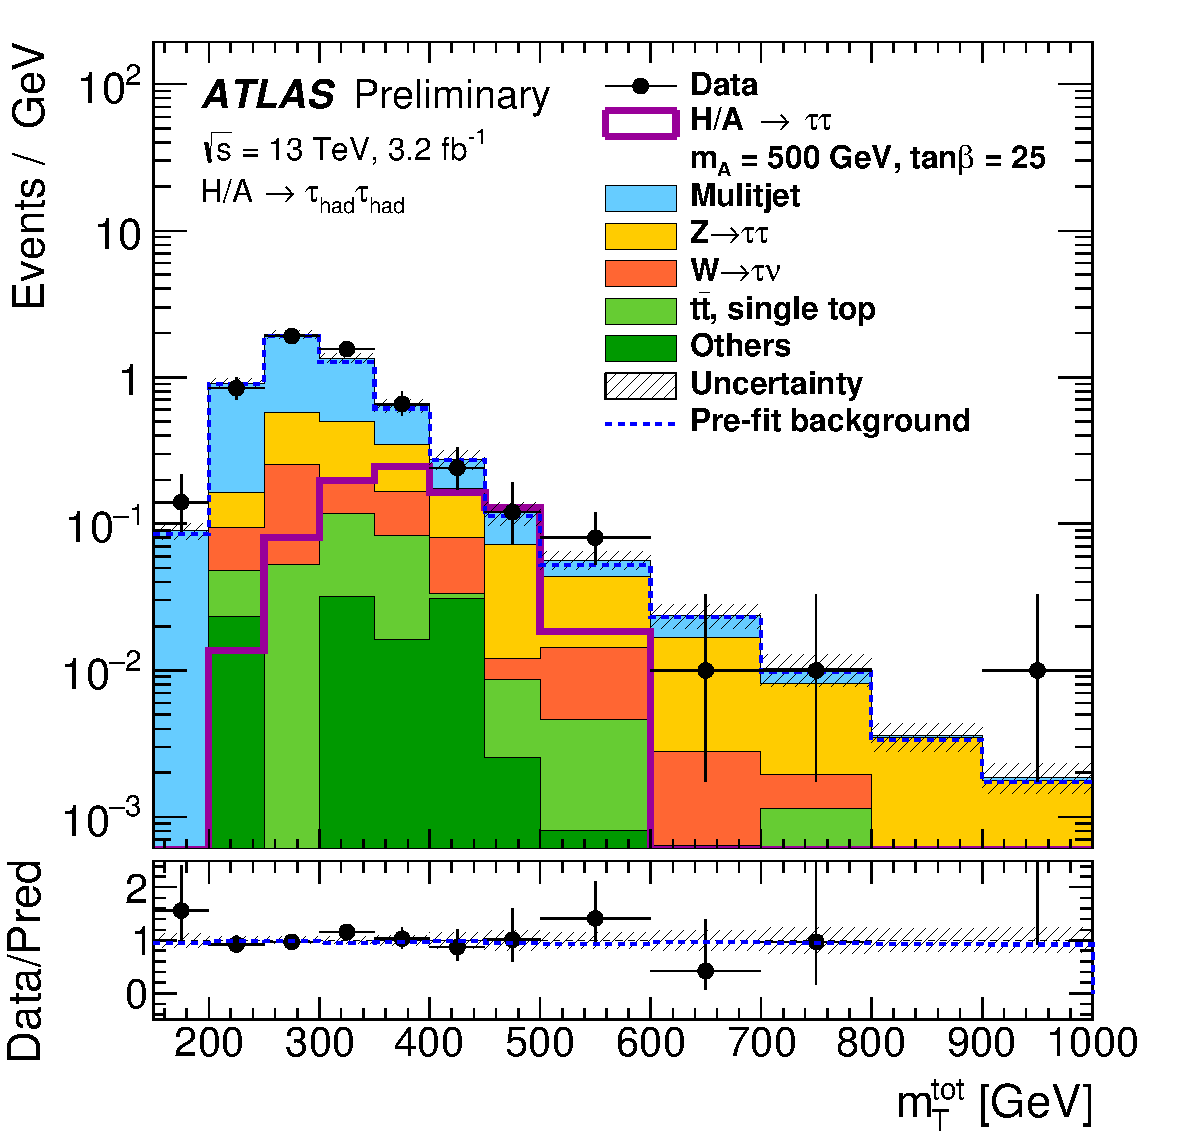
\includegraphics[width=0.45\textwidth, angle=0] {figures/fig_1Htautau_a.pdf}
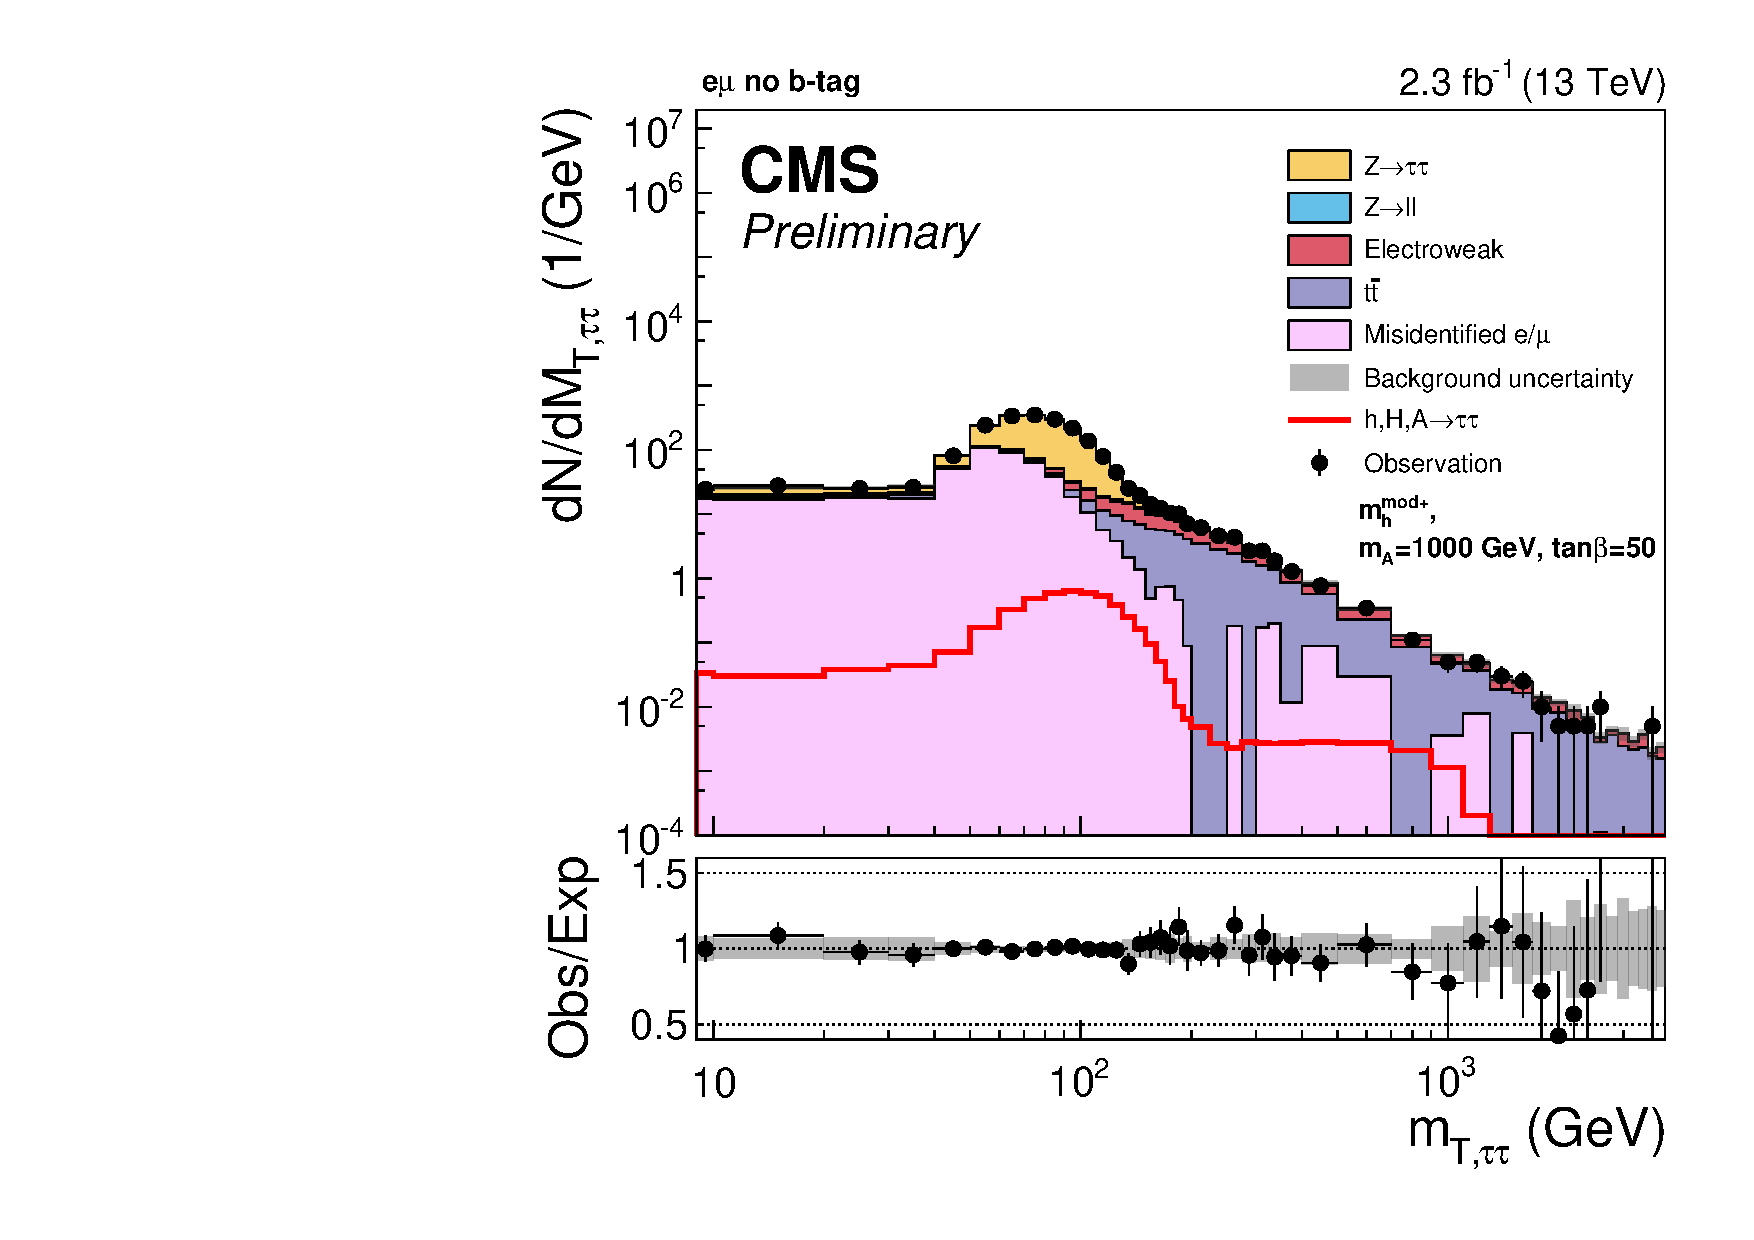
\includegraphics[width=0.45\textwidth, angle=0] {figures/fig_1Htautau_b.pdf}
\caption{ (Left) Post--fit plot of the total transverse mass distribution in f the $\tau_{\rm had}\tau_{\rm had}$ channel by the ATLAS collaboration. (Right) Post--fit plot of the transverse mass distribution in the no b--tag category of the $\tau_{e}\tau_{\mu}$ channel by the CMS collaboration.}
\label{fig_1Htautau}   
\end{figure}

\subsection{Results}
The final result is provided both as a limit on the cross section times branching ratio as well
as a model-dependent limit on various MSSM benchmark models. The limits for all channels combined are shown in Fig. \ref{fig_2aHtautau} and Fig. \ref{fig_2bHtautau}
for the gluon fusion and b-associated production methods respectively, while Fig. \ref{fig_3Htautau} shows the expected and observed 95\% CL upper limits on tan$\beta$ as a function of $m_{A}$ in the MSSM $m_{h}^{mod+}$ scenario, and the comparison with the LHC Run1 results. Already with the  limited statistics recorded in 2015, the sensitivity exceeds the 8 TeV result for $m_{H} >$ 750 GeV for ATLAS and  $m_{H} >$ 350 GeV for CMS. 

\begin{figure}
\centering
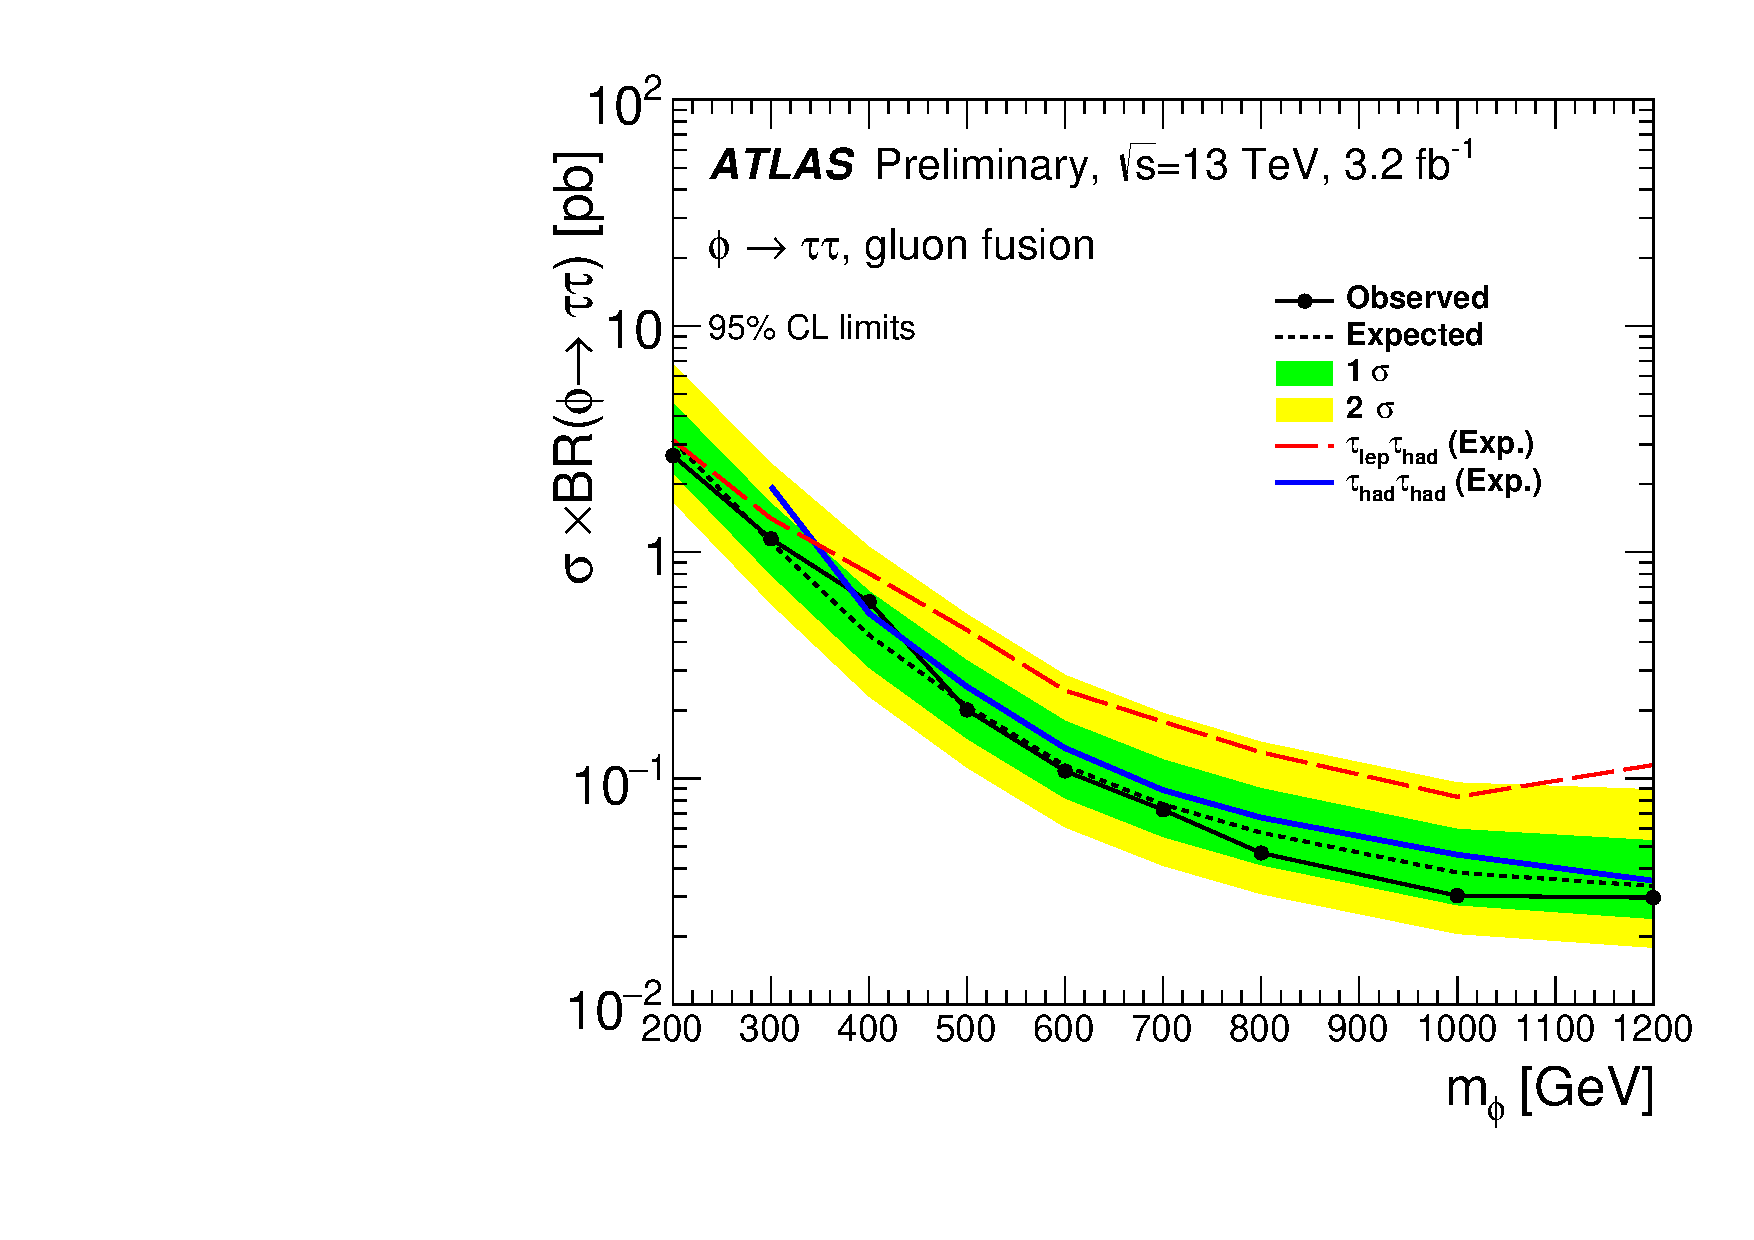
\includegraphics[width=0.45\textwidth, angle=0] {figures/fig_2Htautau_a.pdf}
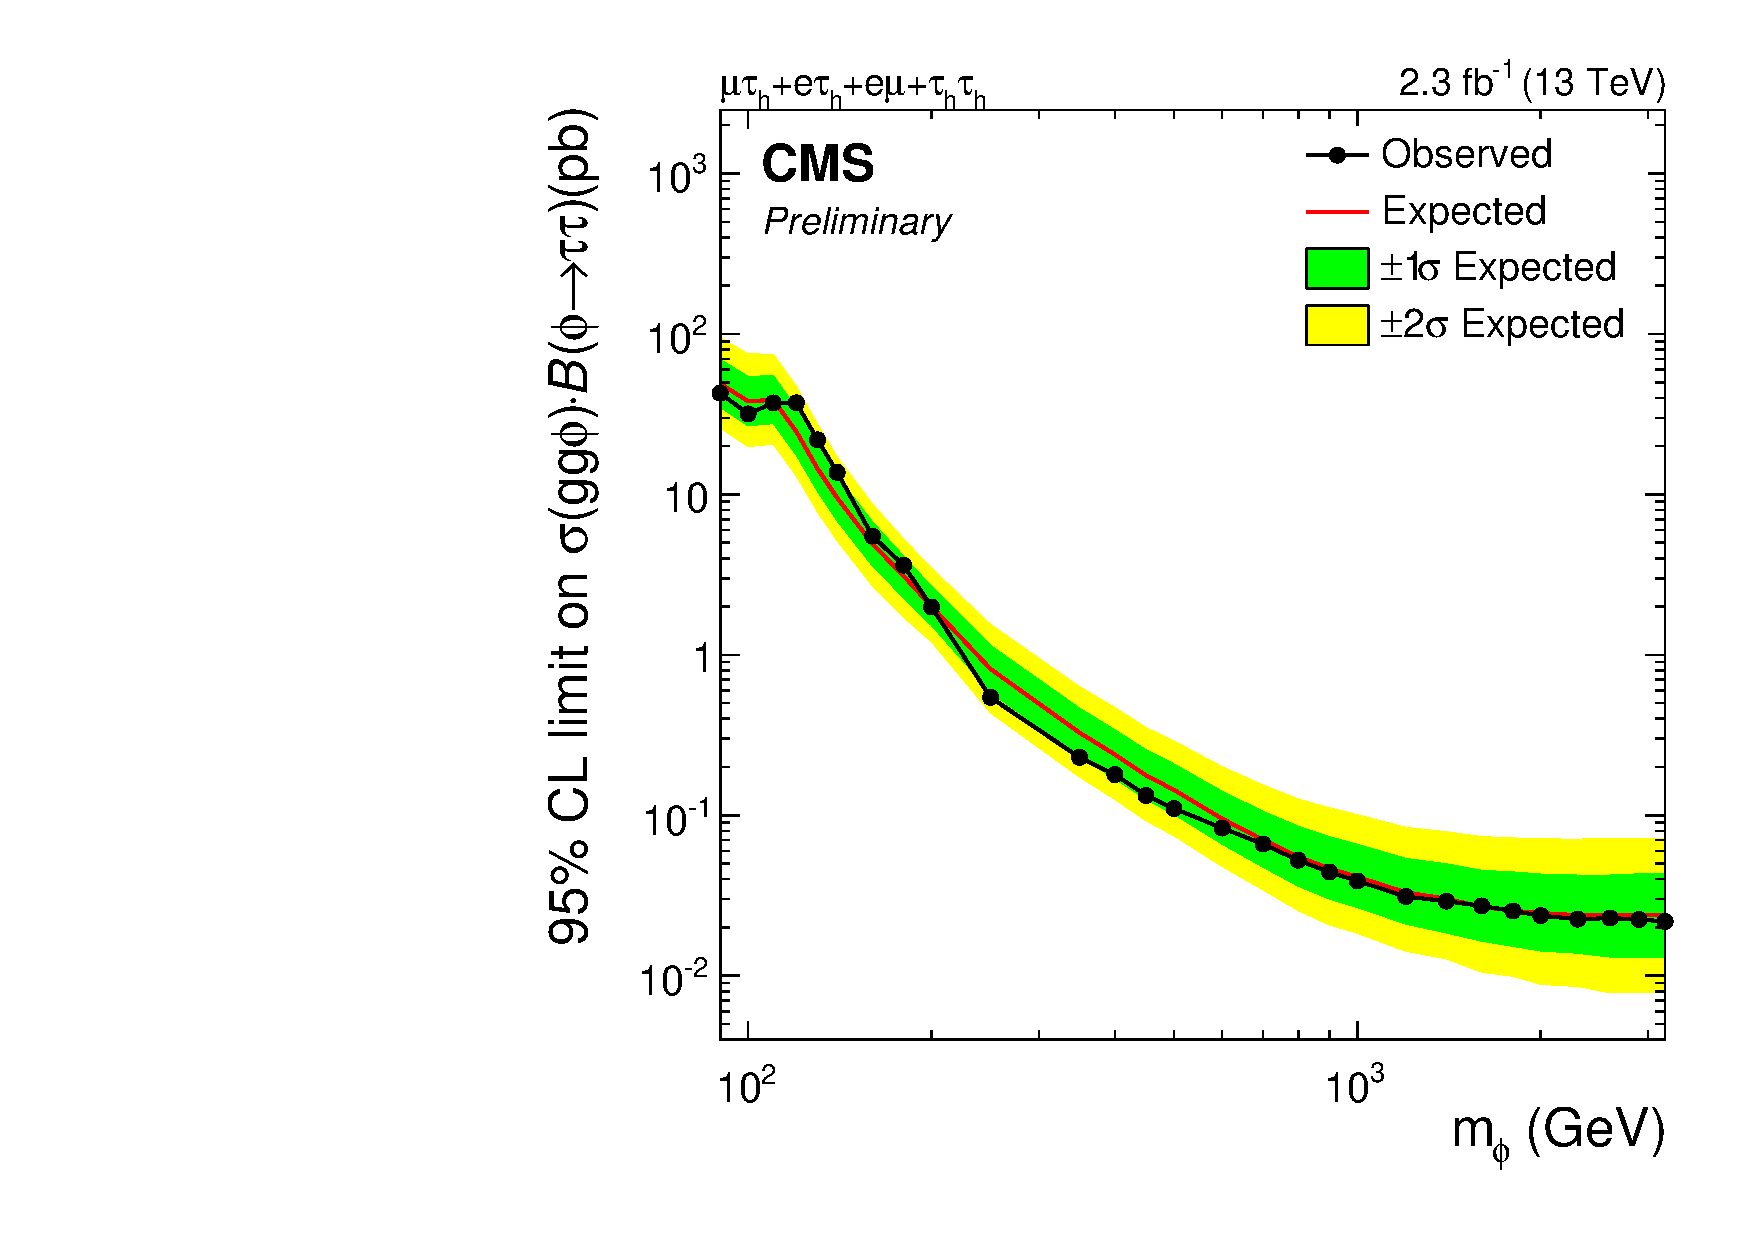
\includegraphics[width=0.45\textwidth, angle=0] {figures/fig_2Htautau_c.pdf}
\caption{ Observed and expected 95\% CL upper limits on the product of cross section and the branching fraction $\sigma(pp\rightarrow \phi) \times B(\phi\rightarrow \tau\tau)$ obtained by the ATLAS collaboriation (left) and by the CMS collaboriation (right) for the gluon-gluon fusion production.}
\label{fig_2aHtautau}   
\end{figure}

\begin{figure}
\centering
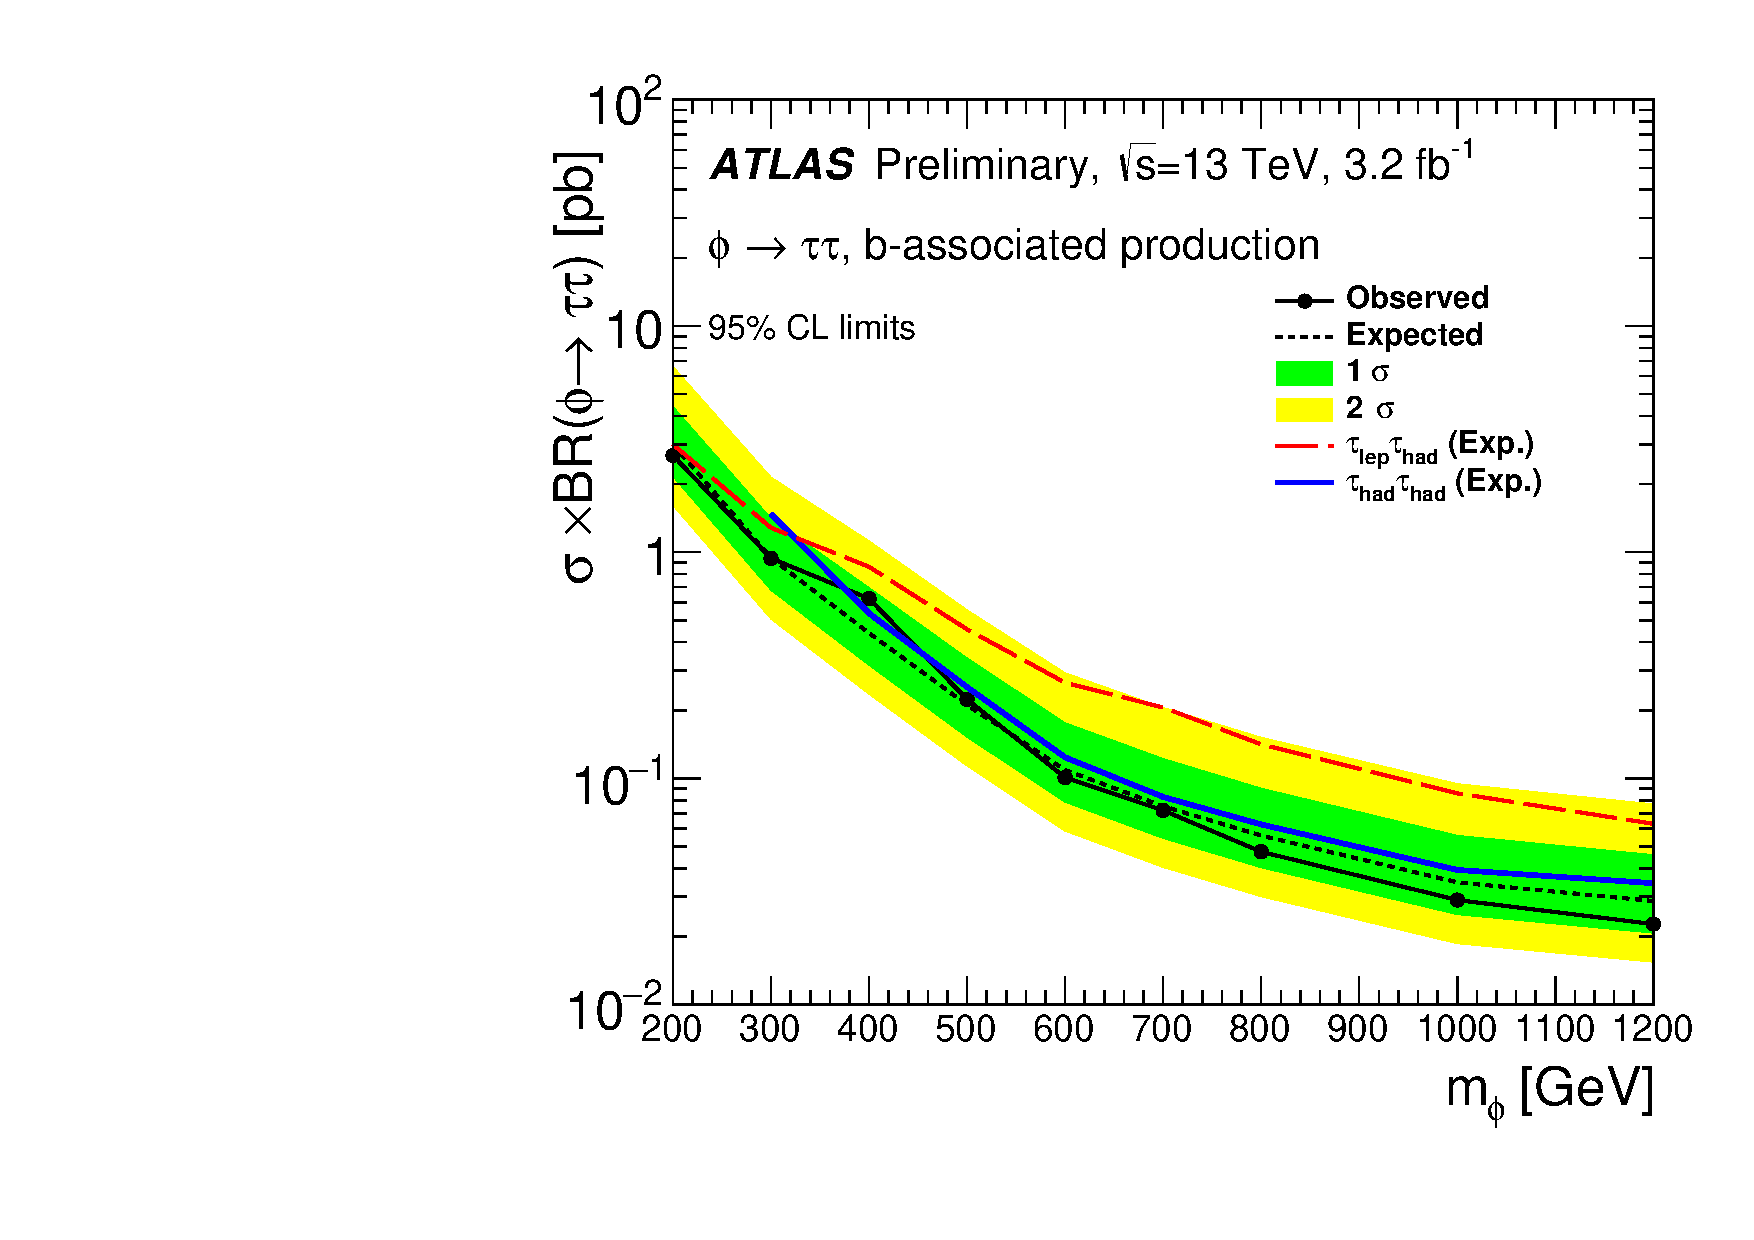
\includegraphics[width=0.45\textwidth, angle=0] {figures/fig_2Htautau_b.pdf}
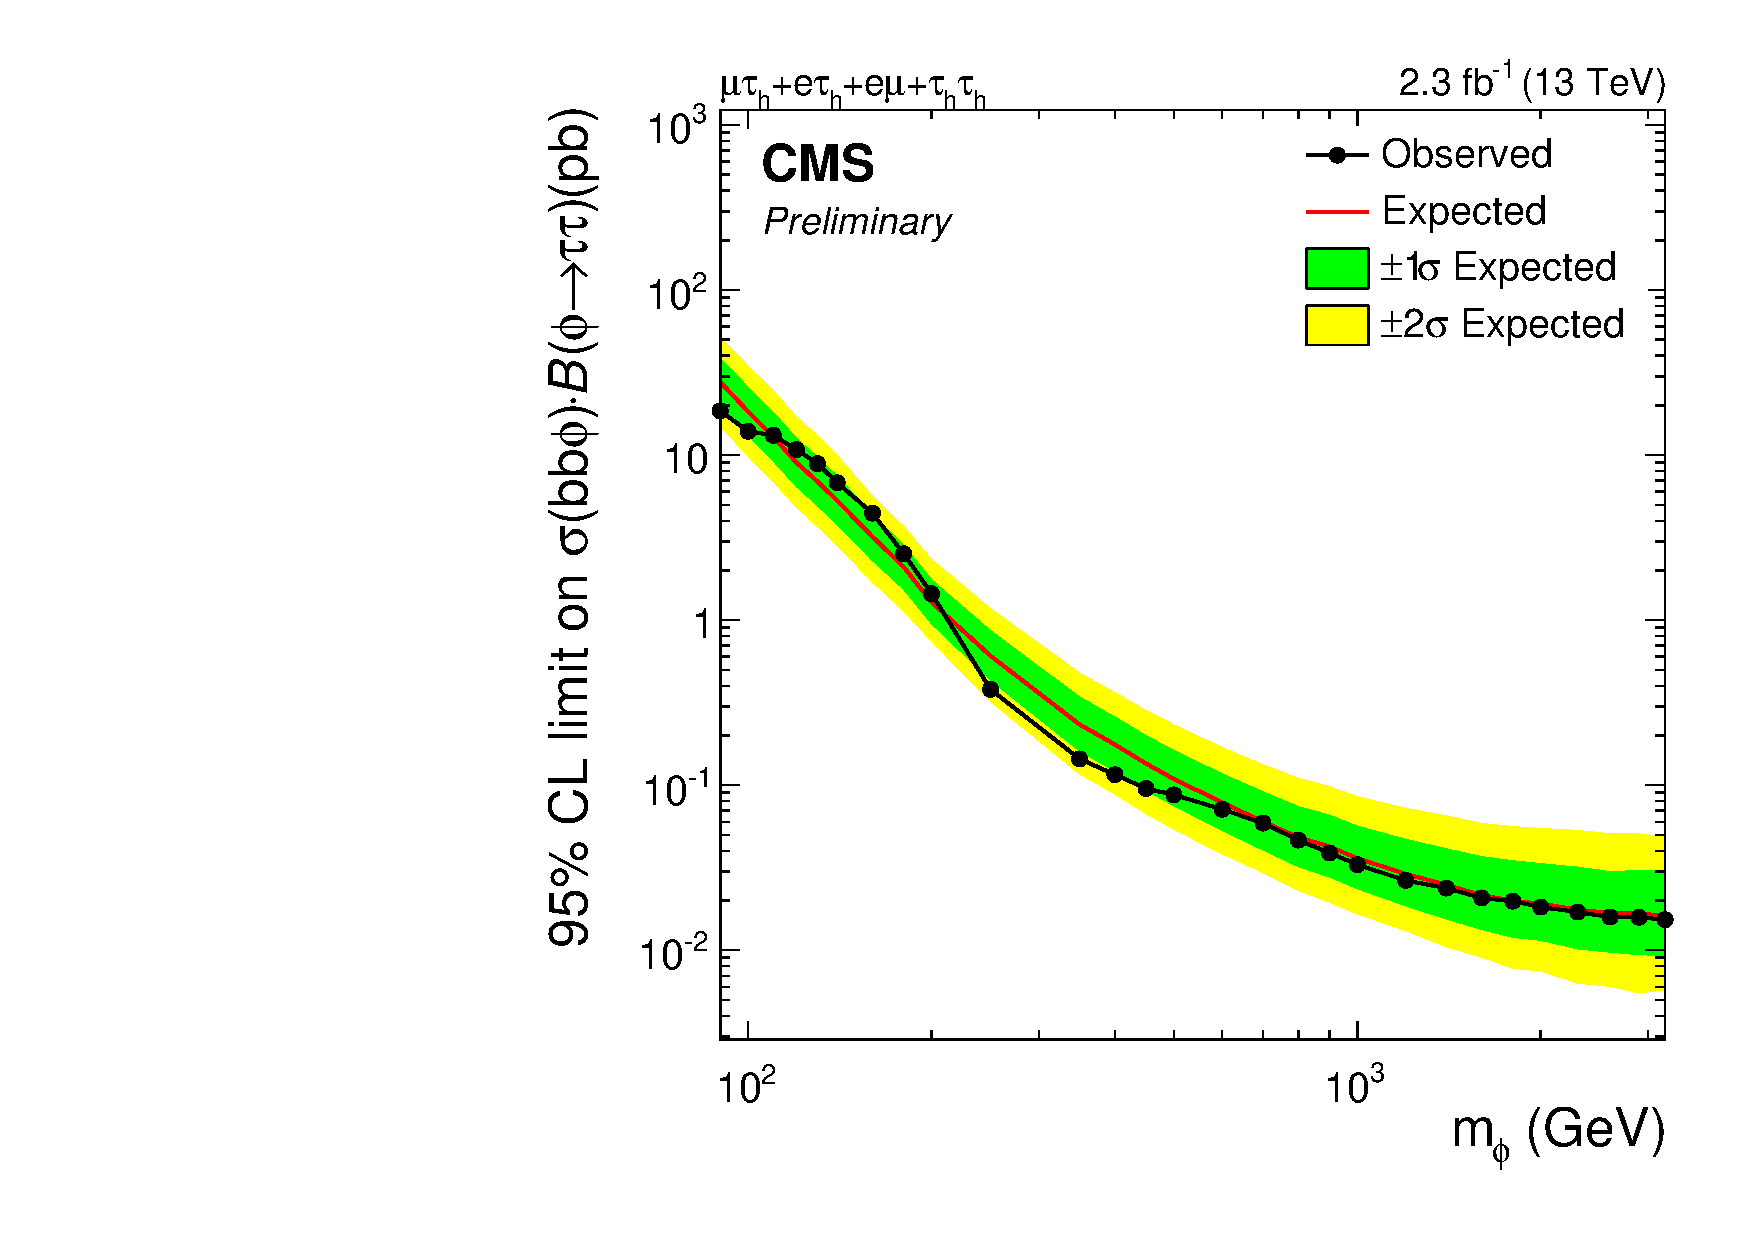
\includegraphics[width=0.45\textwidth, angle=0] {figures/fig_2Htautau_d.pdf}
\caption{ Observed and expected 95\% CL upper limits on the product of cross section and the branching fraction $\sigma(pp\rightarrow \phi) \times B(\phi\rightarrow \tau\tau)$ obtained by the ATLAS collaboriation (left) and by the CMS collaboriation (right) for the b-associted production.}
\label{fig_2bHtautau}   
\end{figure}

\begin{figure}
\centering
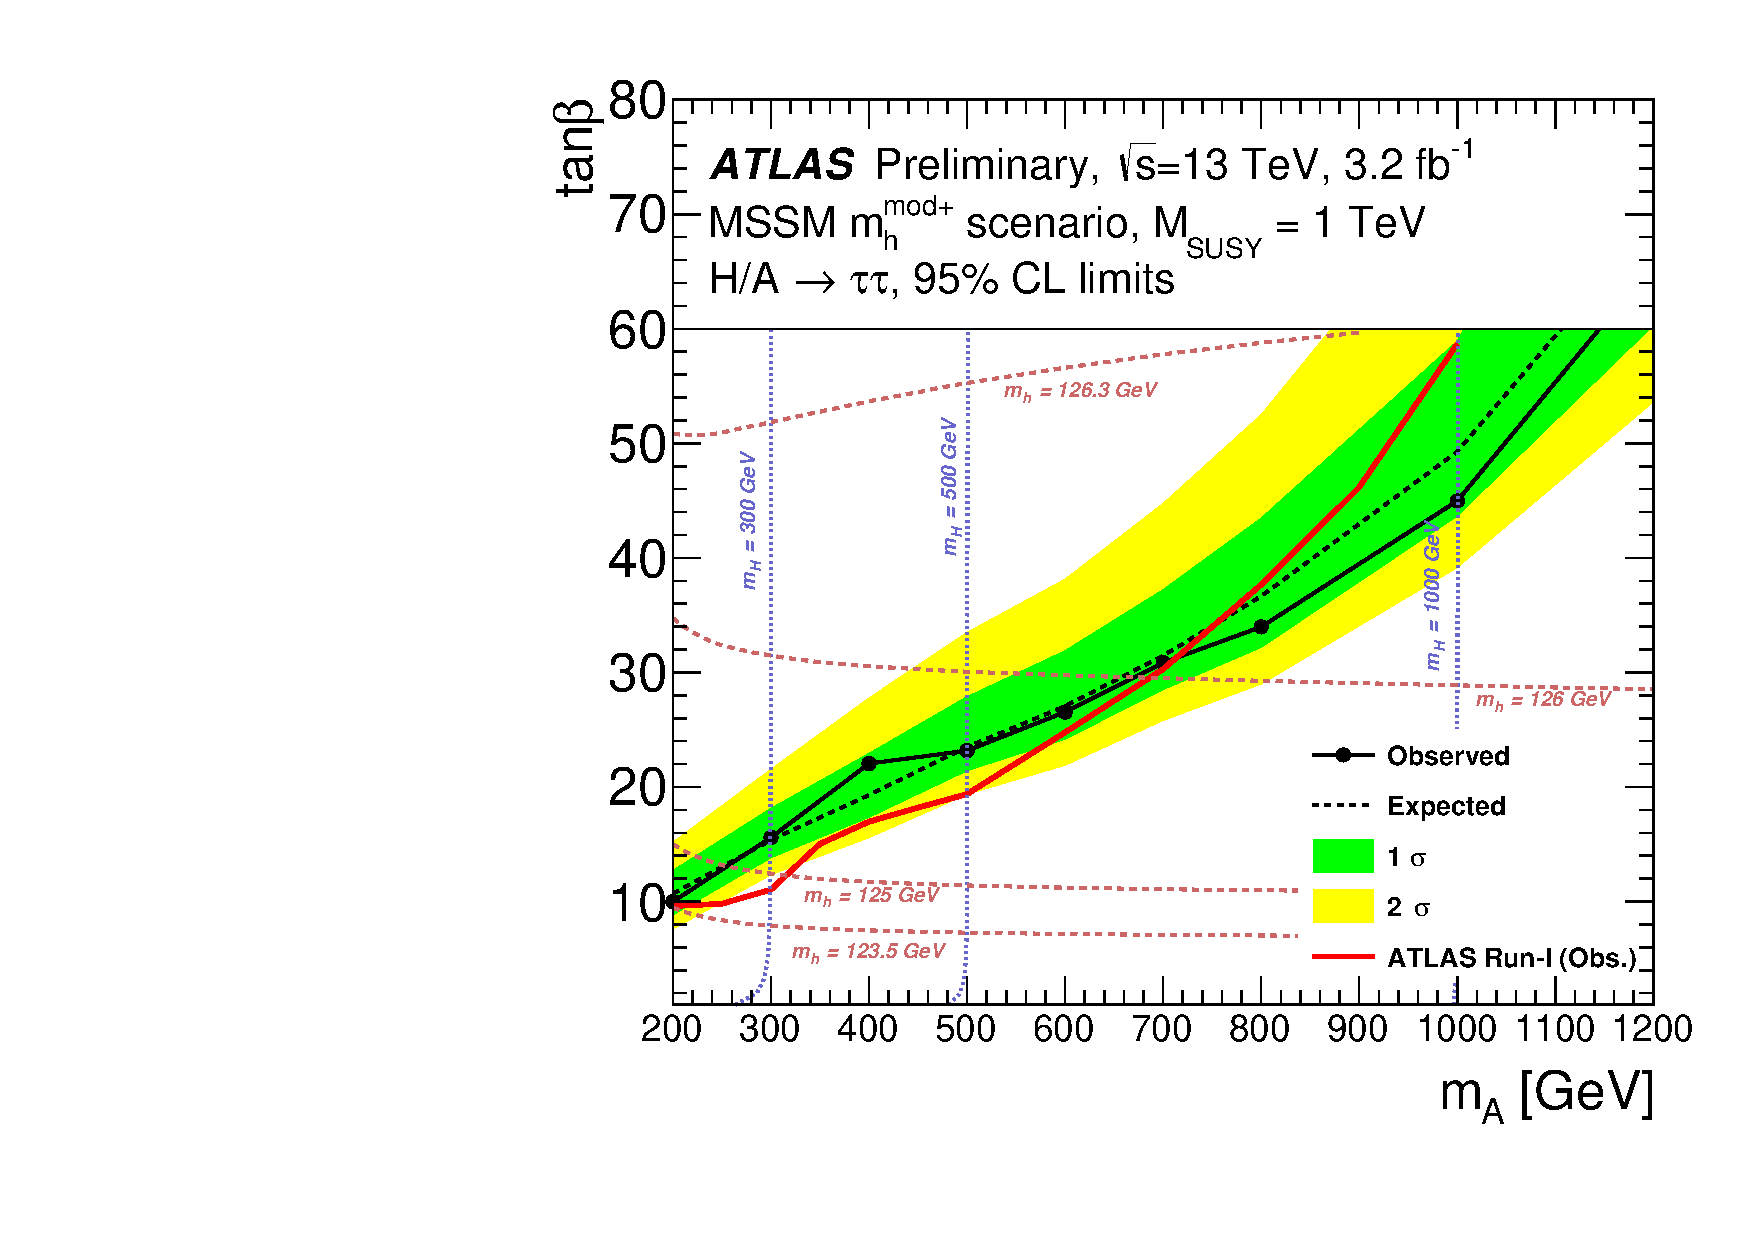
\includegraphics[width=0.45\textwidth, angle=0] {figures/fig_3Htautau_a.pdf}
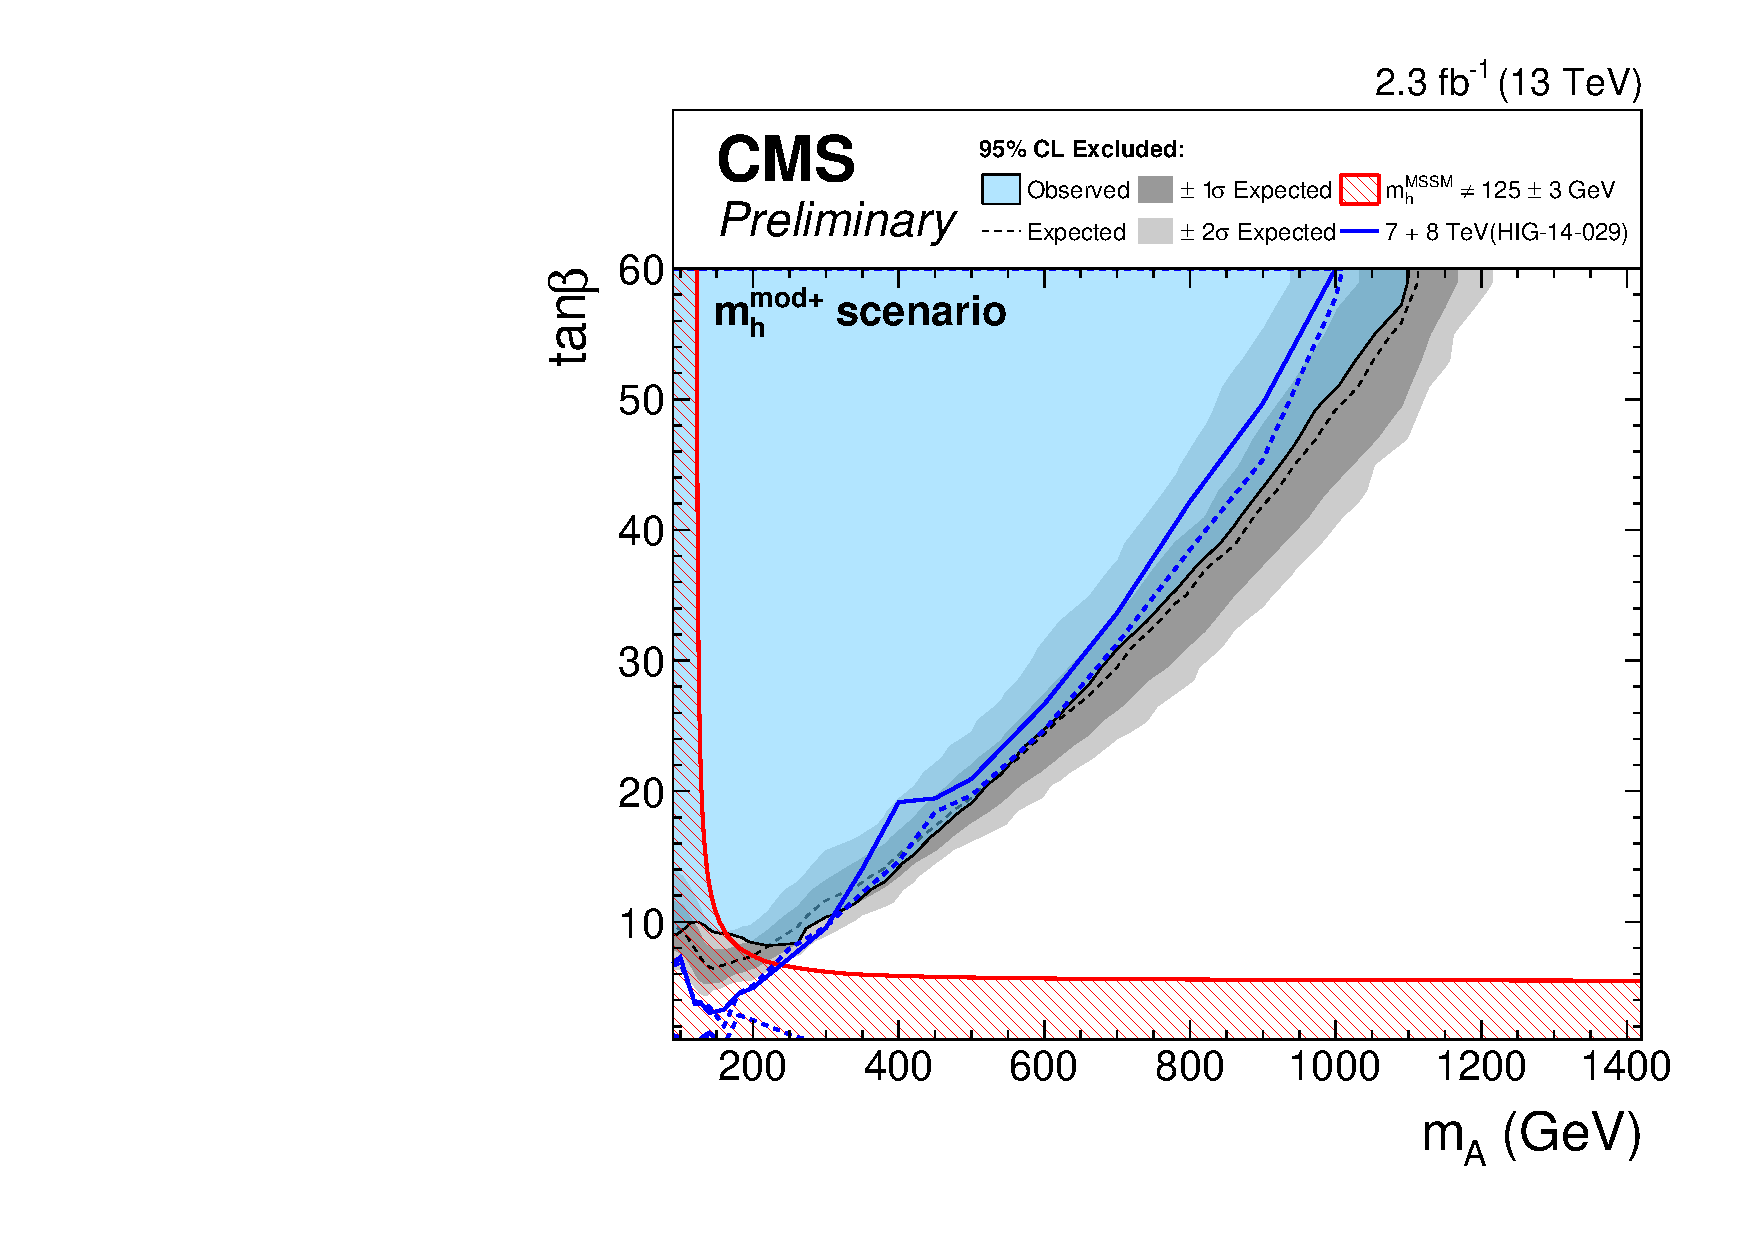
\includegraphics[width=0.45\textwidth, angle=0] {figures/fig_3Htautau_b.pdf}
\caption{ The expected and observed 95\% CL upper limits on tan$\beta$ as a function of $m_{A}$ in the MSSM $m_{h}^{mod+}$ scenario for ATLAS (left) and CMS (right).}
\label{fig_3Htautau}   
\end{figure}

